\subsection{Subsystem $<$Models$>$}

\subsubsection{Detailed Design Diagram}
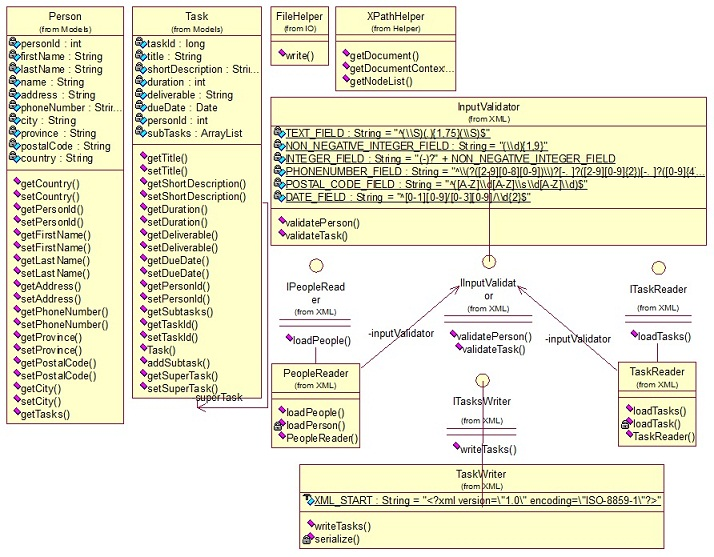
\includegraphics{subsystems/diagrams/models_class_diagram}

This package stores all the classes that belong to the modeling layer of the system. Modeling classes are classes that are used to read and write the data from/to the XML files. It contains the Person, Task, IPeopleReader, PeopleReader, ITaskReader, TaskReader, ITaskWriter, TaskWriter, FileHelper and XPathHelper classes.

\subsubsection{Units Description}

\emph{Person}\\
Functions:\\
\begin{tabular}{| l | l | l | l |}
\hline
Name & Parameters & Pre-conditions & Post-conditions\\
\hline
		String getAddress		& None       			& None			& Returns the address\\
\hline
		String getCity			& None				& None       	 	& Returns the city \\
\hline
		String getCountry		& None				& None       	 	& Returns the country \\
\hline
		String getFirstName		& None				& None       	 	& Returns the firstName \\
\hline
		String getLastName		& None				& None       	 	& Returns the lastName \\
\hline
		String getPersonId		& None				& None       	 	& Returns the personId \\
\hline
		String getPhoneNumber	& None				& None       	 	& Returns the phoneNumber \\
\hline
		String getPostalCode		& None				& None       	 	& Returns the postalCode \\
\hline
		String getProvince		& None				& None       	 	& Returns the province \\
\hline
		ArrayList$<$Task$>$ getTasks		& ArrayList$<$Task$>$ tasks	& Requires the list 	& Returns all the tasks \\
					& 				& of all tasks 		& for this person \\
\hline
		void setAddress		& String address  		& None			& Sets the address\\
\hline
		void setCity			& String city			& None       	 	& Sets the city \\
\hline
		void setCountry		& String country		& None       	 	& Sets the country \\
\hline
		void setFirstName		& String firstName		& None       	 	& Sets the firstName \\
\hline
		void setLastName		& String lastName		& None       	 	& Sets the lastName \\
\hline
		void setPersonId		& String personId		& None       	 	& Sets the personId \\
\hline
		void setPhoneNumber	& String phoneNumber	& None       	 	& Sets the phoneNumber\\
\hline
		void setPostalCode		& String postalCode		& None       	 	& Sets the postalCode\\
\hline
		void setProvince		& String province		& None       	 	& Sets the province
\\
\hline
\end{tabular}
\\

Attributes:\\
\begin{tabular}{| l | l |}
\hline
 Name                                       & Description\\
\hline
String address		 	 & Address of this person\\
\hline
String city		 	 & City of this person\\
\hline
String country		 	 & Country of this person\\
\hline
String firstName		  & First name of this person\\
\hline
String lastName		  & Last name of this person\\
\hline
String personId		  & Id of this person\\
\hline
String phoneNumber		  & Phone number of this person\\
\hline
String postalCode		  & Postal code of this person\\
\hline
String province		  & Province of this person\\
\hline
\end{tabular}\\
\\

Purpose: Its purpose is to hold the information that is read from the XML file for a particular person.
\\
\\

\emph{Task}\\
Functions:\\
\begin{tabular}{| l | l | l | l |}
\hline
Name & Parameters & Pre-conditions & Post-conditions\\
\hline
		Task				& None       			& None			& Default constructor, \\
						& 	       			& 			& initializes subtasks \\
\hline
		void addSubtask		& Task task			& None       	 	& Adds subtask to this task \\
\hline
		String getDeliverable		& None				& None       	 	& Returns the deliverable \\
\hline
		String getDueDate		& None				& None       	 	& Returns the dueDate \\
\hline
		String getDuration		& None				& None       	 	& Returns the duration \\
\hline
		String getPersonId		& None				& None       	 	& Returns the person Id \\
\hline
		String getShortDescription	& None				& None       	 	& Returns the short description \\
\hline
		String getSubtasks		& None				& None       	 	& Returns the subtasks list \\
\hline
		String getSuperTask		& None				& None       	 	& Returns the super task \\
\hline
		String getTaskId		& None		  		& None			& Returns the task Id \\
\hline
		String getTitle			& None				& None       	 	& Returns the title \\
\hline
		void setDeliverable		& String deliverable		& None       	 	& Sets the deliverable \\
\hline
		void setDueDate		& String dueDate		& None       	 	& Sets the dueDate \\
\hline
		void setDuration		& String duration		& None       	 	& Sets the duration \\
\hline
		void setPersonId		& String personId		& None       	 	& Sets the personId\\
\hline
		void setShortDescription	& String shortDescription	& None       	 	& Sets the shortDescription\\ 
\hline
		void setSuperTask		& String superTask		& None       	 	& Sets the superTask \\
\hline
		void setTaskId			& String taskId	  		& None			& Sets the taskId \\
\hline
		void setTitle			& String title			& None       	 	& Sets the title
\\
\hline
\end{tabular}
\\

Attributes:\\
\begin{tabular}{| l | l |}
\hline
 Name                                     	 	& Description\\
\hline
String deliverable			& Deliverable of this task\\
\hline
String dueDate			& Due date of this task\\
\hline
String duration		 		& Duration of this task\\
\hline
String personId			& ID of the person this task belongs to\\
\hline
String shortDescription		& Short description of this task\\
\hline
ArrayList$<$Task$>$ subTasks	& Sub-tasks of this task\\
\hline
String superTask			& Super task of this task\\
\hline
\end{tabular}\\
\\

Purpose: Its purpose is to hold the information that is read from the XML file for a particular task and its sub-tasks. If the object has a superTask, then this task is a subtask of that superTask.
\\
\\

\emph{IPeopleReader}\\
Functions:\\
\begin{tabular}{| l | l | l | l |}
\hline
Name & Parameters & Pre-conditions & Post-conditions\\
\hline
		ArrayList$<$Person$>$loadPeople 	& String path       			& Requires the path 	& Returns the list of people\\
                                                                                    &                         			 & to the people XML file	& 
\\
\hline
\end{tabular}
\\

Purpose: The interface for loading the people XML file.
\\
\\
\emph{PeopleReader}\\
Functions:\\
\begin{tabular}{| l | l | l | l |}
\hline
Name & Parameters & Pre-conditions & Post-conditions\\
\hline
		PeopleReader				& IInputValidator 	& None				& Default constructor, \\
							& inputValidator	&  requires inputValidator	& \\
\hline
		ArrayList$<$Person$>$loadPeople 	& String path       	& Requires the path,		& Returns all people\\
                                                                                    &                         	& returns a list of people 	 &\\
\hline
		Person loadPerson 			& JXPathContext path & Requires the context	& Returns a Person \\
                                                                                    & personCtx                & pointer			& 
\\
\hline
\end{tabular}
\\

Attributes:\\
\begin{tabular}{| l | l |}
\hline
 Name                                     	 	& Description\\
\hline
IInputValidator inputValidator		& Input validator for reading the XML file\\
\hline
\end{tabular}\\
\\

Purpose: Its purpose is load all the people from the specified XML file path.
\\
\\

%%%%%%%%%%%%%%%%%%%%%%%%%%%%%%
\emph{ITaskReader}\\
Functions:\\
\begin{tabular}{| l | l | l | l |}
\hline
Name & Parameters & Pre-conditions & Post-conditions\\
\hline
		ArrayList$<$Task$>$loadTasks 	& String path       			& Requires the path 	& Returns the list of task\\
                                                                                    &                         			 & to the tasks XML file	& 
\\
\hline
\end{tabular}
\\

Purpose: The interface for loading the tasks XML file.
\\
\\
\emph{TaskReader}\\
Functions:\\
\begin{tabular}{| l | l | l | l |}
\hline
Name & Parameters & Pre-conditions & Post-conditions\\
\hline
		TaskReader				& IInputValidator 	& None				& Default constructor, \\
							& inputValidator	&  requires inputValidator	& \\
\hline
		ArrayList$<$Task$>$loadTasks 	& String path       	& Requires the path,		& Returns all tasks\\
                                                                                    &                         	& returns a list of taks 	 &\\
\hline
		Task loadTask	 			& JXPathContext path & Requires the context	& Returns a Task \\
                                                                                    & taskCtx                	& pointer			& 
\\
\hline
\end{tabular}
\\

Attributes:\\
\begin{tabular}{| l | l |}
\hline
 Name                                     	 	& Description\\
\hline
IInputValidator inputValidator		& Input validator for reading the XML file\\
\hline
\end{tabular}\\
\\

Purpose: Its purpose is load all the taks from the specified XML file path.
\\
\\

%%%%%%%%%%%%%%%%%%%%%%%%%%%%%%
\emph{ITasksWriter}\\
Functions:\\
\begin{tabular}{| l | l | l | l |}
\hline
Name & Parameters & Pre-conditions & Post-conditions\\
\hline
		boolean writeTasks 	& String path       			& Requires the path 		& Returns a flag to\\
                                                           & 					& to the tasks XML file		& indicate if save \\
\hline
                                                           & ArrayList$<$Task$>$ tasks		& Requires list	of tasks	& was succesful
\\
\hline
\end{tabular}
\\

Purpose: The interface for writing the tasks XML file.
\\
\\
\emph{TasksWriter}\\
Functions:\\
\begin{tabular}{| l | l | l | l |}
\hline
Name & Parameters & Pre-conditions & Post-conditions\\
\hline
		boolean writeTasks 			& String path       			& Requires the path		& Returns a flag to indicate \\
                                                                                    & ArrayList$<$Task$>$ tasks             & and list of tasks 		 &  if save was succesful \\
\hline
		String serialize 			& ArrayList$<$Task$>$ tasks		& Requires list of tasks	& Returns serialized tasks
\\
\hline
\end{tabular}
\\

Attributes: \emph{none}

Purpose: Its purpose is write all the taks to the specified XML file path.
\\
\\

%%%%%%%%%%%%%%%%%%%%%%%%%%%
\emph{XPathHelper}\\
Functions:\\
\begin{tabular}{| l | l | l | l |}
\hline
Name & Parameters & Pre-conditions & Post-conditions\\
\hline
		Document getDocument 		& Object xmlFile       			& Requires the an object	& Returns the XML\\
                                                                                    & 				             & than can be the filepath    	& document \\
							& 					& or an InputStream		& \\
\hline
		Document getDocumentContext	& Object xmlFile       			& Requires the an object	& Returns the XML \\
                                                                                    & 				             & than can be the filepath    	& JXPathContext \\
							& 					& or an InputStream		& \\
\hline
		NodeList getNodeList			& Document doc       			& Requires this XML 		 & Returns the list \\
                                                                                    & String query			            & document and a    		& of nodes matching \\
							& 					& query for nodes		& the specified query
\\
\hline
\end{tabular}
\\

Attributes: \emph{none}

Purpose: Its purpose is load and query any XML file in memory.
\\
\\